%%%%%%%%%%%%%%%%%%%%%%%%%%%%%%%%%%%%%%%%%%%%%%
%                insertmeeting
% 1) Title (something creative & funny?)
% 2) Date (MM/DD/YYYY)
% 3) Location (ex. Hagerty High School)
% 4) People/Committees Present 
% 5) Picture 
% 6) Start Time & Stop Time (ex. 12:30AM to 4:30PM)
%%%%%%%%%%%%%%%%%%%%%%%%%%%%%%%%%%%%%%%%%%%%%%
\insertmeeting 
	{Drippy Driving} 
	{12/08/21} 
	{Hagerty High School}
	{Jensen}
	{Images/RobotPics/robot.jpg}
	{2:30 - 4:30}
	
\hhscommittee{General}
\noindent\hfil\rule{\textwidth}{.4pt}\hfil
\subsubsection*{Goals}
\begin{itemize}
    \item Do driver practice
    \item Use software to improve driving experience
 

\end{itemize} 

\noindent\hfil\rule{\textwidth}{.4pt}\hfil

\subsubsection*{Accomplishments}
Although we have been meeting less because of our semester exams, we have still been able to fit in some driver practice when our software team isn’t working on autonomous. Recently, we have been getting much better at driving and are feeling like we understand what each other are doing much better than before. Because this is the first year where we have had more than a couple days of driver practice before competitions, we have been very surprised at how much better we have been able to get. We have also found new ways to improve the driving experience through software that we may have otherwise never thought of. One thing that we recently changed was making the robot automatically slow down when turning. Because we used to have to slow down during turning manually, we lost some time slowing down during the straight sections where we can go fast to prepare for a turn. Because the robot does this for us automatically, it makes driving the robot and making turns flow much better and allows us to add a whole new cycle to our teleop period. Thanks to lots of practice and changes like this, we were able to score our new personal best of 8 elements on the alliance shipping hub (1 on mid and 7 on top) for a total of 46 points (Figure \ref{fig:120821_1})! Although we don't think we will score quite this high at the meet because of increased stress and less than perfect conditions, we still feel that we will do better driving than at our first meet.

 
\begin{figure}[htp]
\centering
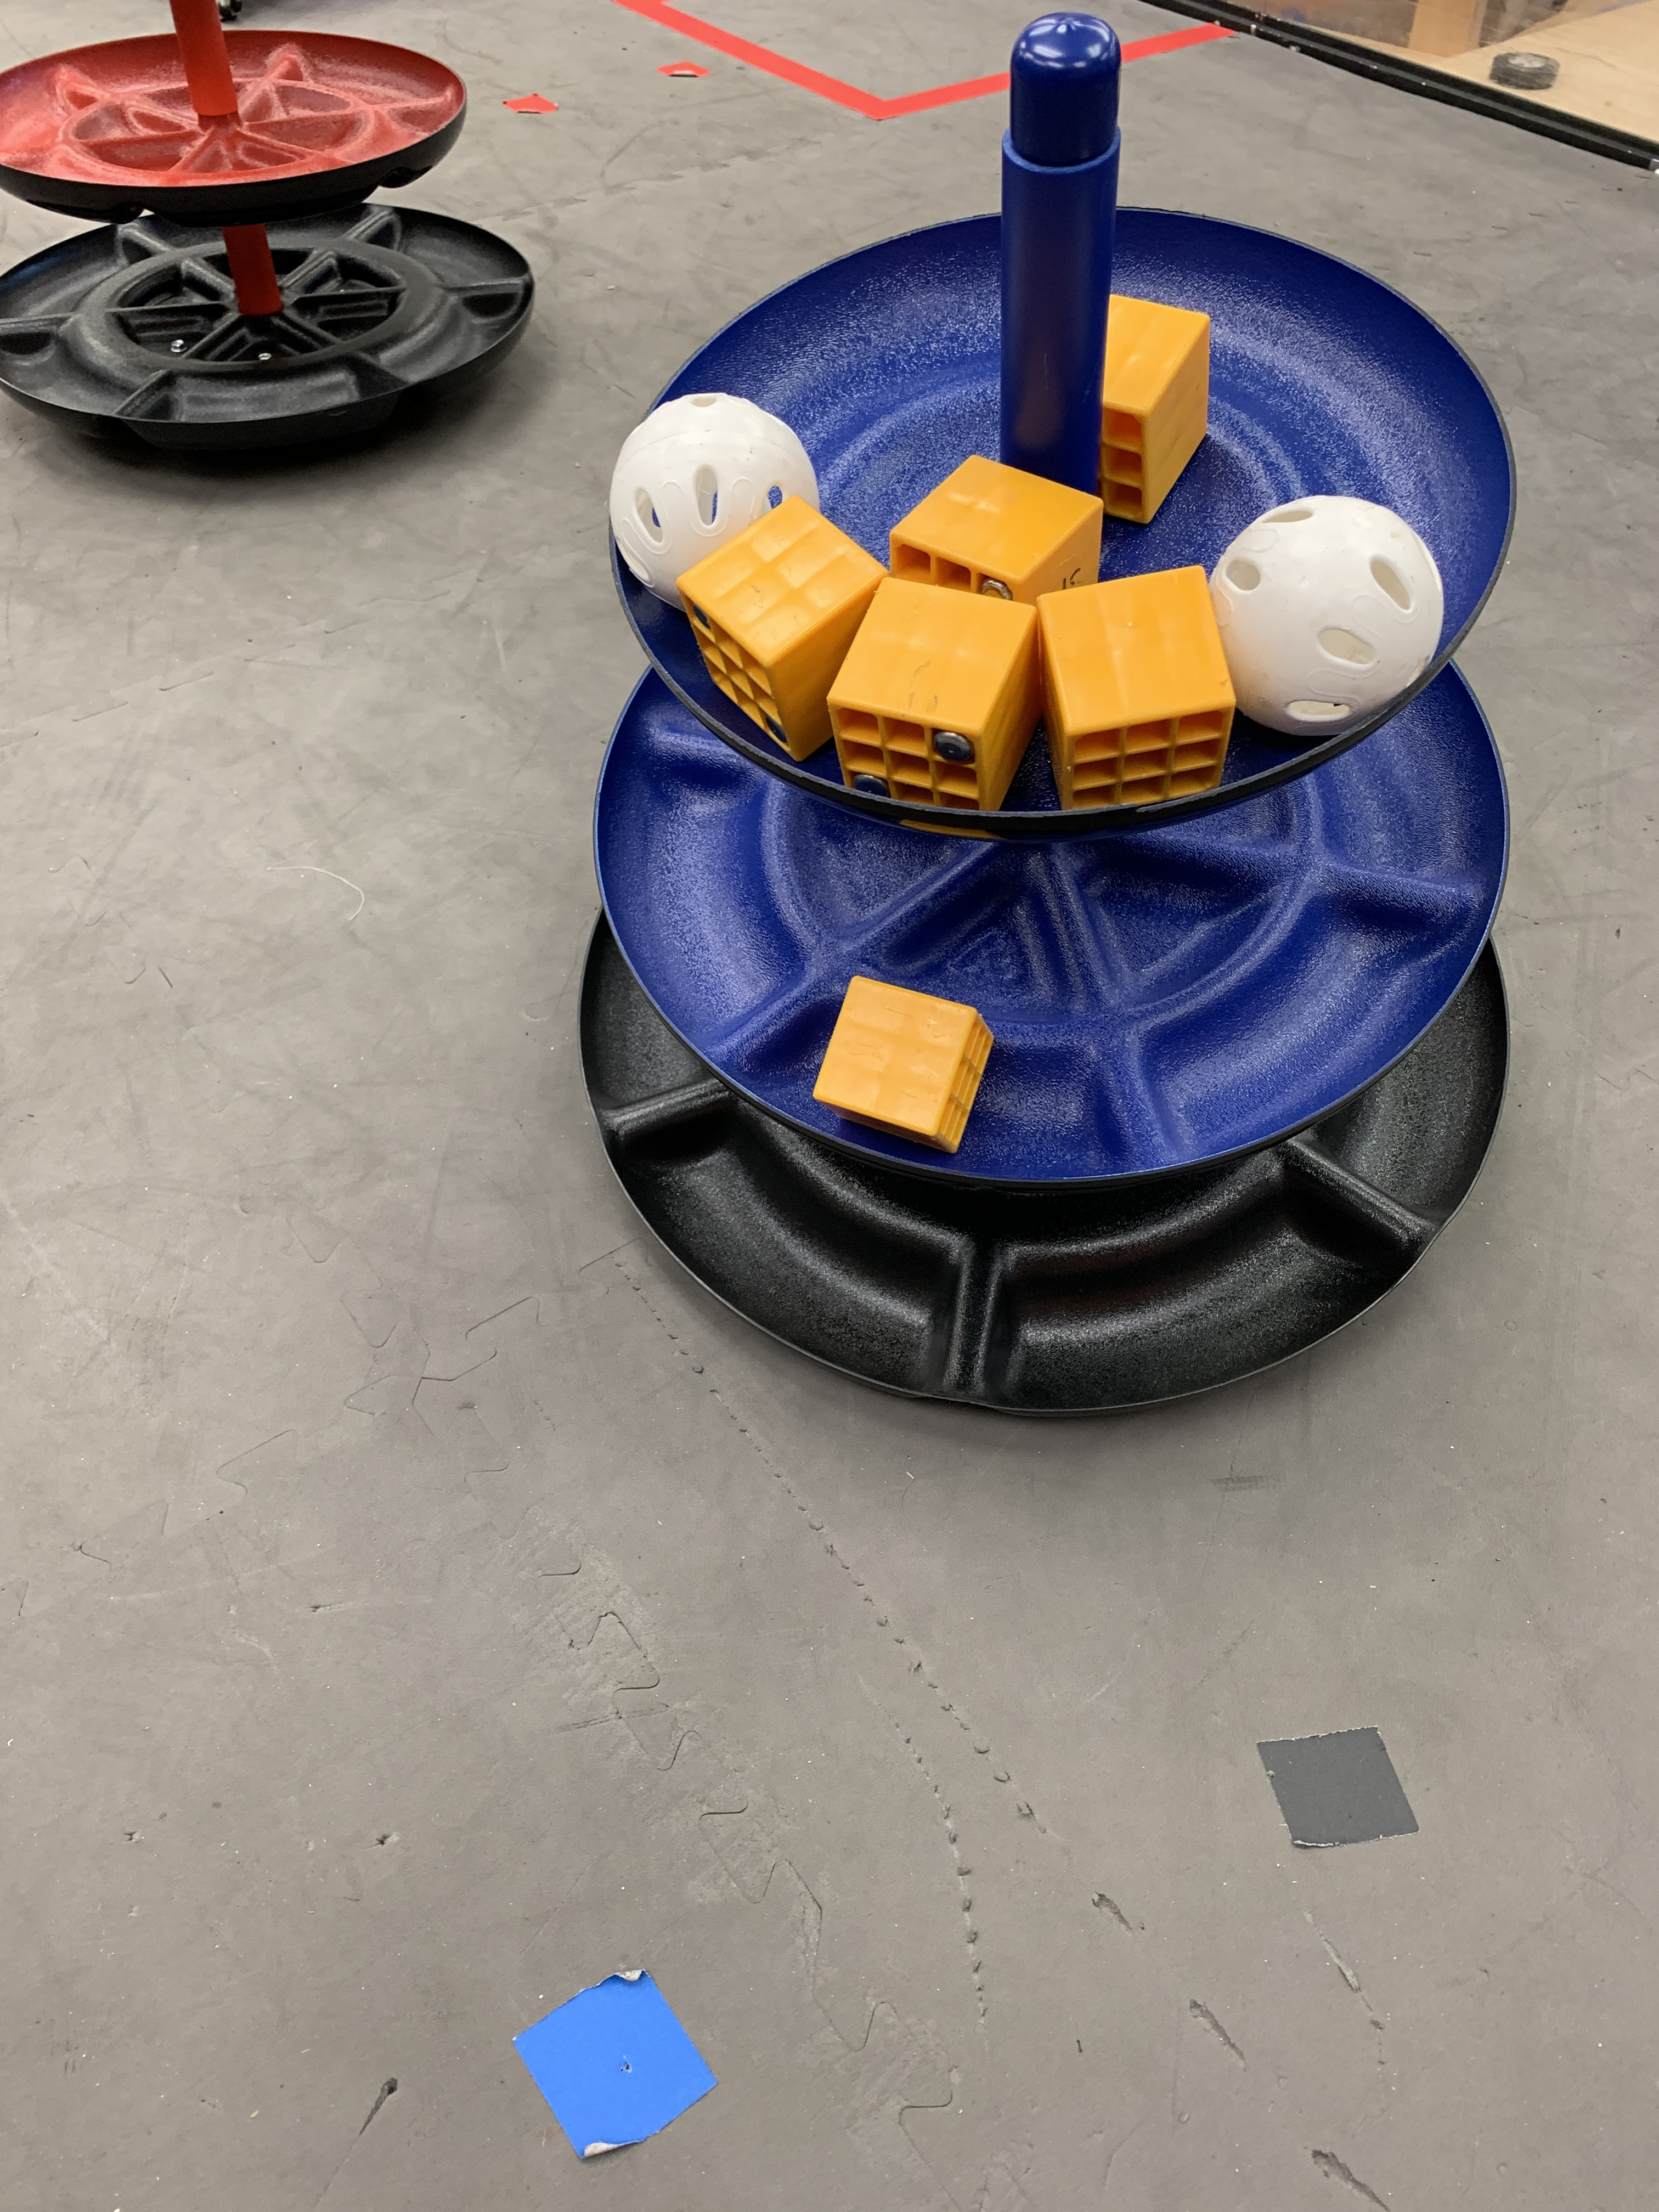
\includegraphics[width=0.95\textwidth, angle=0]{Meetings/December/12-08-21/12-8-21_Team_Figure1 - Nathan Forrer.JPG}
\caption{The alliance shipping hub}
\label{fig:120821_1}
\end{figure}


\whatsnext{
\begin{itemize}
    \item Keep practicing driving
    \item Continue preparing for upcoming meet

\end{itemize} 
}

